
\documentclass[preprint,12pt]{elsarticle}

\usepackage[spanish]{babel}
\usepackage{amssymb}
\usepackage{graphicx}
\usepackage{lineno}
\usepackage[utf8]{inputenc}
\usepackage{url}
\usepackage{natbib} 
\usepackage{amsmath} 
\usepackage{amssymb} 
\usepackage{multicol}

\begin{document}
	
\begin{titlepage}
\centering
	{
\includegraphics[width=0.2\textwidth]{./IMAGENES/upt}\par}
	\vspace{1cm}
	{\bfseries\LARGE Universidad Privada de Tacna\par}
	\vspace{1cm}
	{\scshape\Large Escuela Profesional de Ingenieria de Sistemas \par}
	\vspace{2cm}
	{\scshape\LARGE Aplicación biométrica basada en web para la autenticacion de usuarios \par}
	\vspace{2cm}
	{\large Integrantes: Franklin Huichi Contreras, Jose Pastor Mendoza \par}
	\vspace{0.1cm}
	{\large Ciclo: Octavo Ciclo \par}
	\vspace{0.1cm}
	{\large Curso: Seguridad Informatica \par}
	\vspace{0.1cm}
	{\large Docente: Ing. Oscar Jimenez Flores\par}
	\vfill
	{\large Tacna - Perú 2020 \par}

\end{titlepage}

\begin{multicols}{2} 

%% Desarrollo ----------------------------------------------------------------------------------------------------------------
\section{Desarrollo} 
La biometría es una tecnología que puede identificar a una persona en función de sus características físicas. La identificación y el reconocimiento de huellas digitales es un método biométrico que se usa ampliamente en varios tipos de aplicaciones debido a su precisión y confiabilidad. El objetivo principal de este proyecto es analisar un sistema que pueda reconocer si 2 impresiones provienen de la misma persona o no. Con este fin, las imágenes se recopilan primero de un conjunto de datos. Luego, sobre las mismas imágenes, se aplican técnicas de procesamiento de imágenes digitales para mejorar su calidad. Una vez que la imagen se se limpie se encuentra los puntos críticos que luego se comparan según su distancia de Hamming.

\subsection{¿ Como se realizo ?} 
	\subsubsection{Limpiamos la imagen del ruido} Para la limpiaza de la imagen y las crestas de la huella se usa una libreria llamada enhance la cual segun su documentacion "Utiliza un banco de filtros gabor orientado para mejorar la imagen de la huella digital. La orientación de los filtros gabor se decide por la orientación de las crestas en la imagen de entrada." todo ello para mejorar una imagen de huella digital. \\
En terminos faciles de entender usa la frecuencia en puntos especificos, en regiones localizadas alrededor del punto o region de analisis para poder eliminar la menor frecuencia y dejar la mayor freceuncia encontrada en la imagen, en donde la menor frecuencia es denominada ruido. \\

{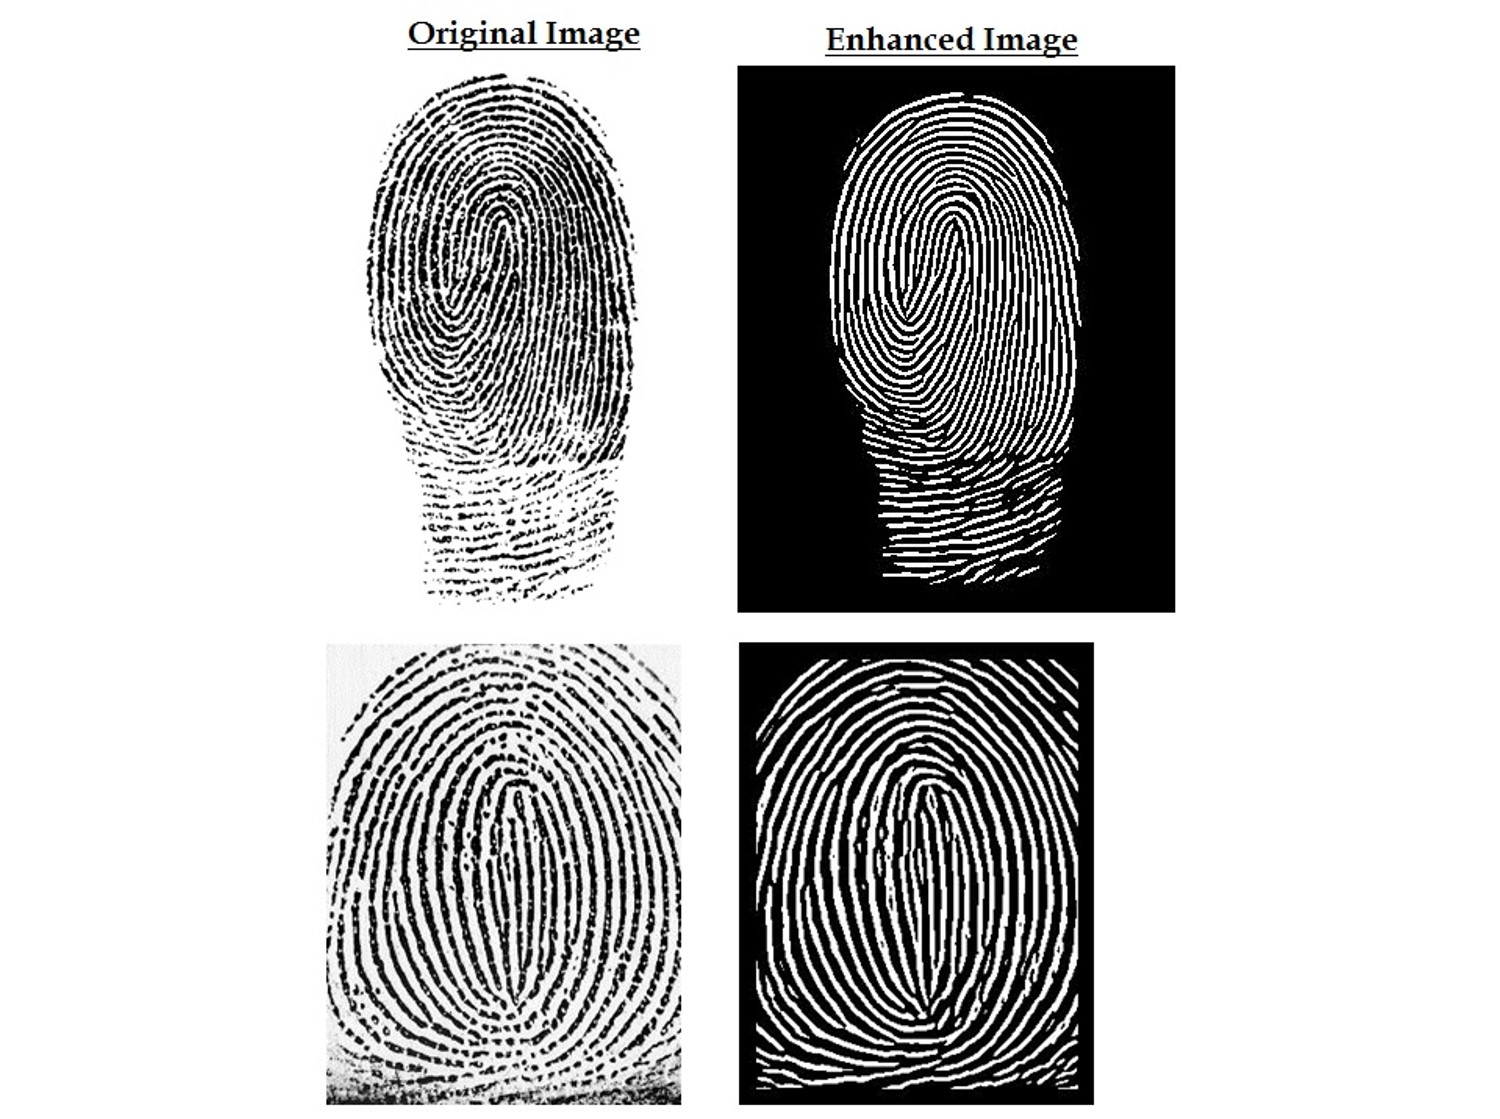
\includegraphics[width=0.5\textwidth]{./IMAGENES/ruido}\par}

	\subsubsection{Escogemos el mejor umbral con otsu} 
El umbral de Otsu seleccionará automáticamente el mejor umbral genérico para la imagen para obtener un buen contraste entre la información de primer plano y de fondo. \\

{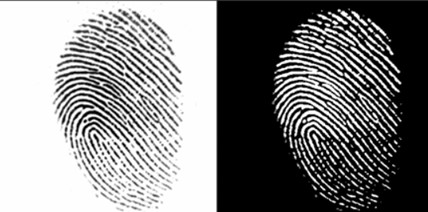
\includegraphics[width=0.4\textwidth]{./IMAGENES/otsu}\par}

	\subsubsection{Esquetelizamos la huella} 
Para mejorar el proceso de búsqueda de puntos críticos en la huella digital, es bueno esqueletizar la imagen en sí. Esto crea puntos críticos más únicos y más fuertes.\\

{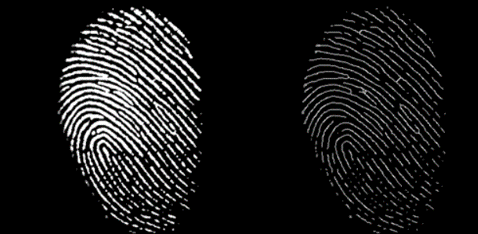
\includegraphics[width=0.4\textwidth]{./IMAGENES/esqueleto}\par}

	\subsubsection{Detectar puntos criticos}
Una vez que se obtiene la imagen esquelética, el siguiente paso sería encontrar puntos para cruzar las crestas de la impresión, que luego se llaman puntos minuciosos. Esto se puede hacer con la ayuda de un detector de punto crítico, que requiere un cambio importante en el contraste local. Tal es el detector Harris Corner. Debido a que el detector Harris Corner es capaz de detectar ángulos y bordes fuertes, esto es ideal para el problema de la huella digital, donde los mínimos más importantes son bordes cortos y bifurcaciones, en donde las posiciones donde se juntan los bordes.  \\

{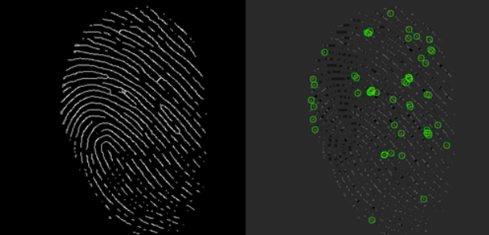
\includegraphics[width=0.4\textwidth]{./IMAGENES/harris}\par}

\subsubsection{Unir los puntos y calcular igualdades}
Después de obtener la matriz de descriptores para dos impresiones, se necesita un algoritmo para compararlas. La forma que se usa es la distancia de Hamming entre los descriptores de 2 puntos diferentes. De esta manera obtendremos una puntuación que indica qué tan similares son esas 2 impresiones. Establecer un umbral puede determinar si las impresiones son iguales o no.
	\subsubsection{Pruebas de codigo}
	
{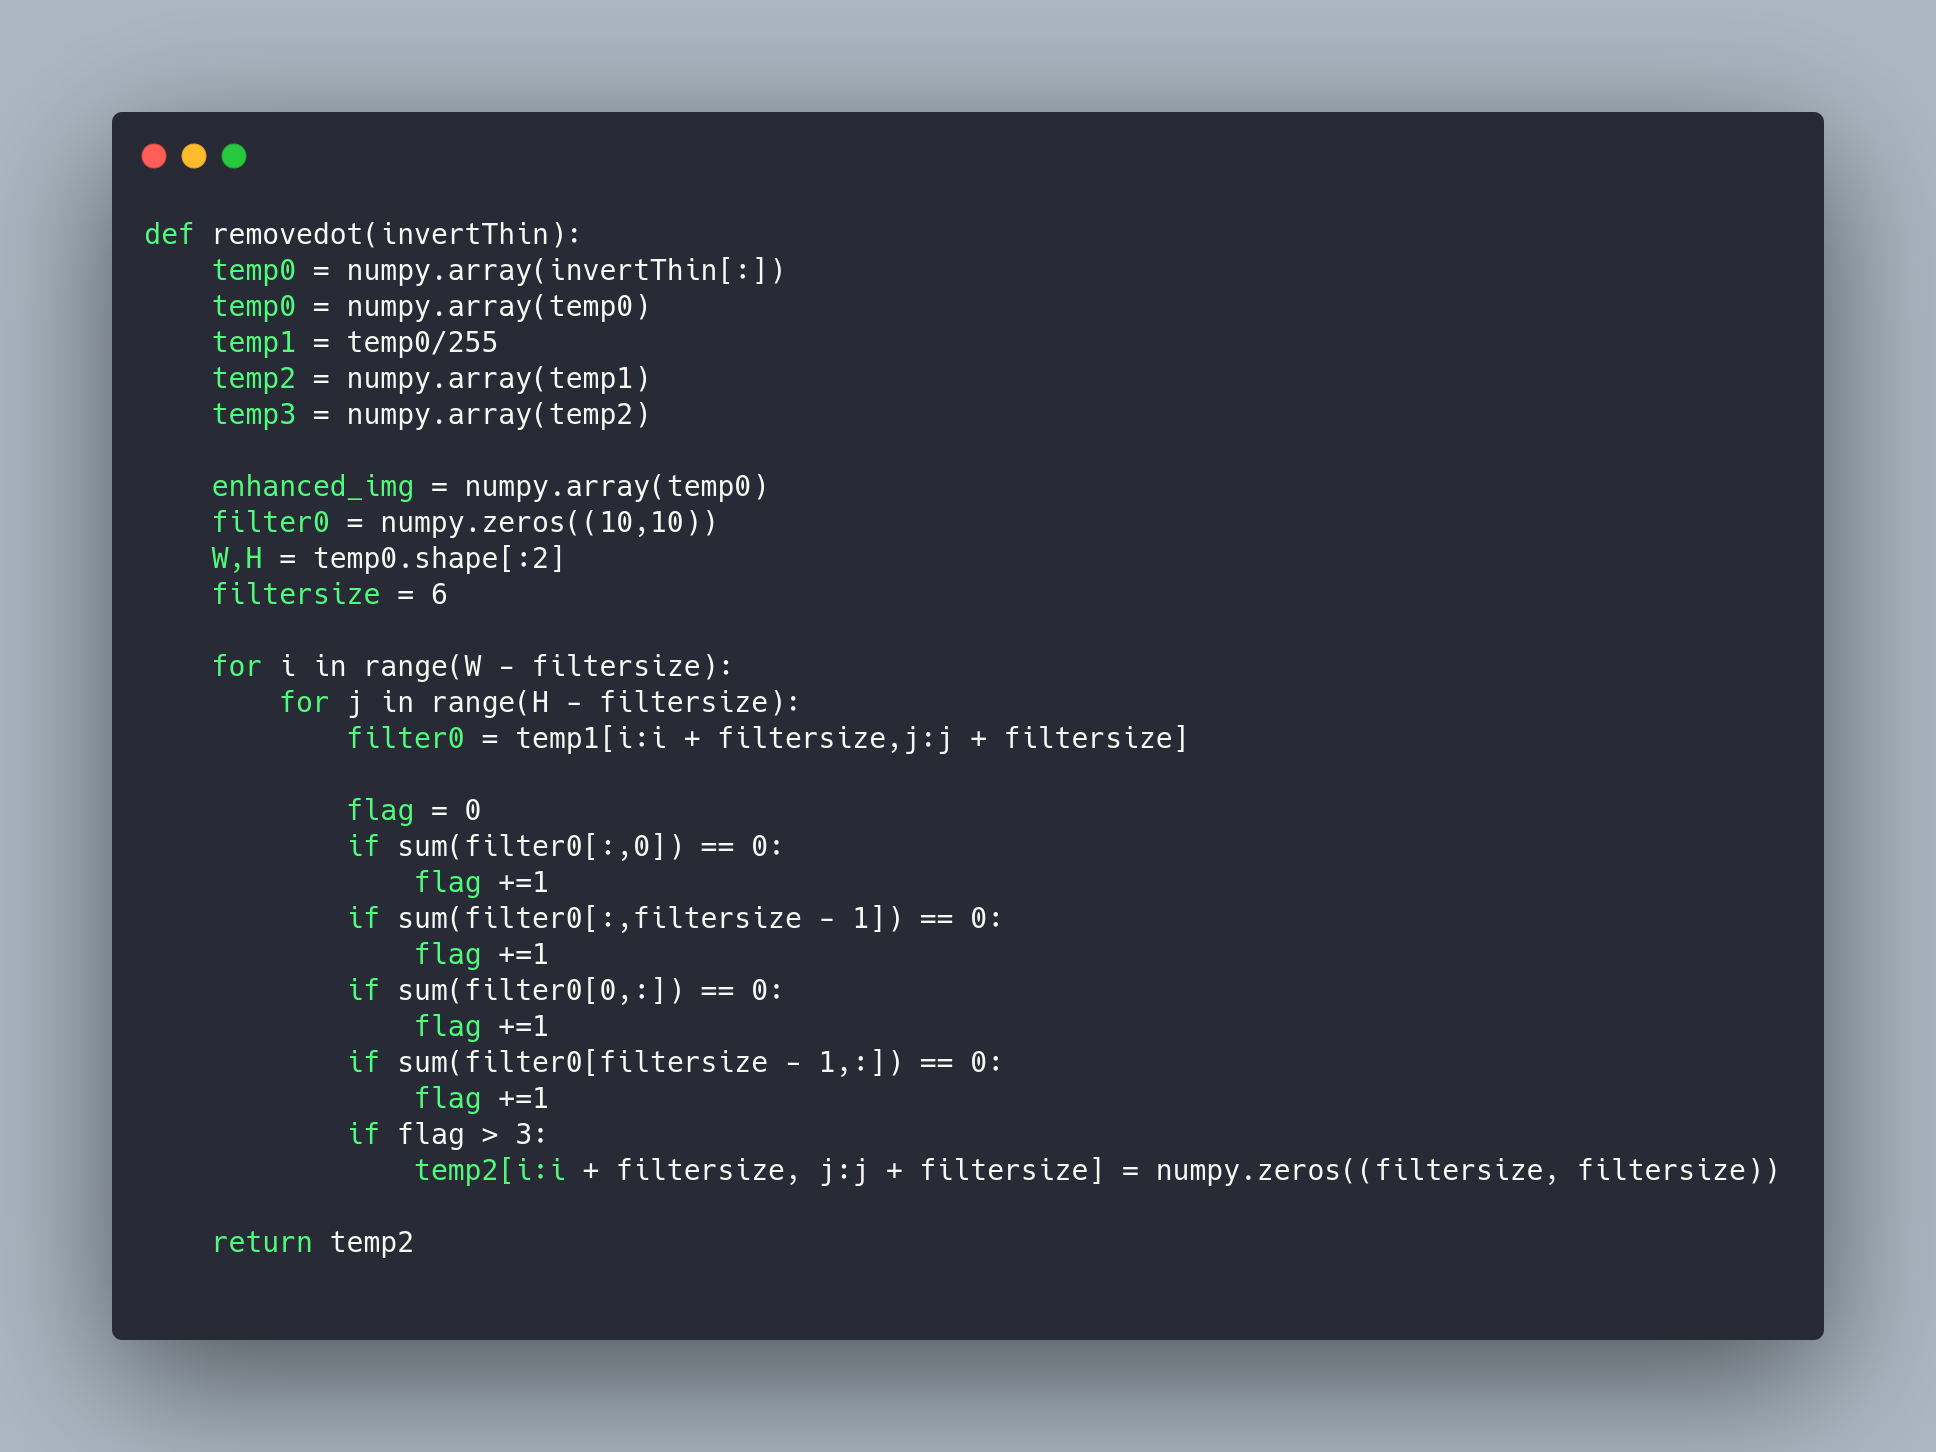
\includegraphics[width=0.4\textwidth]{./IMAGENES/removedot}\par}
{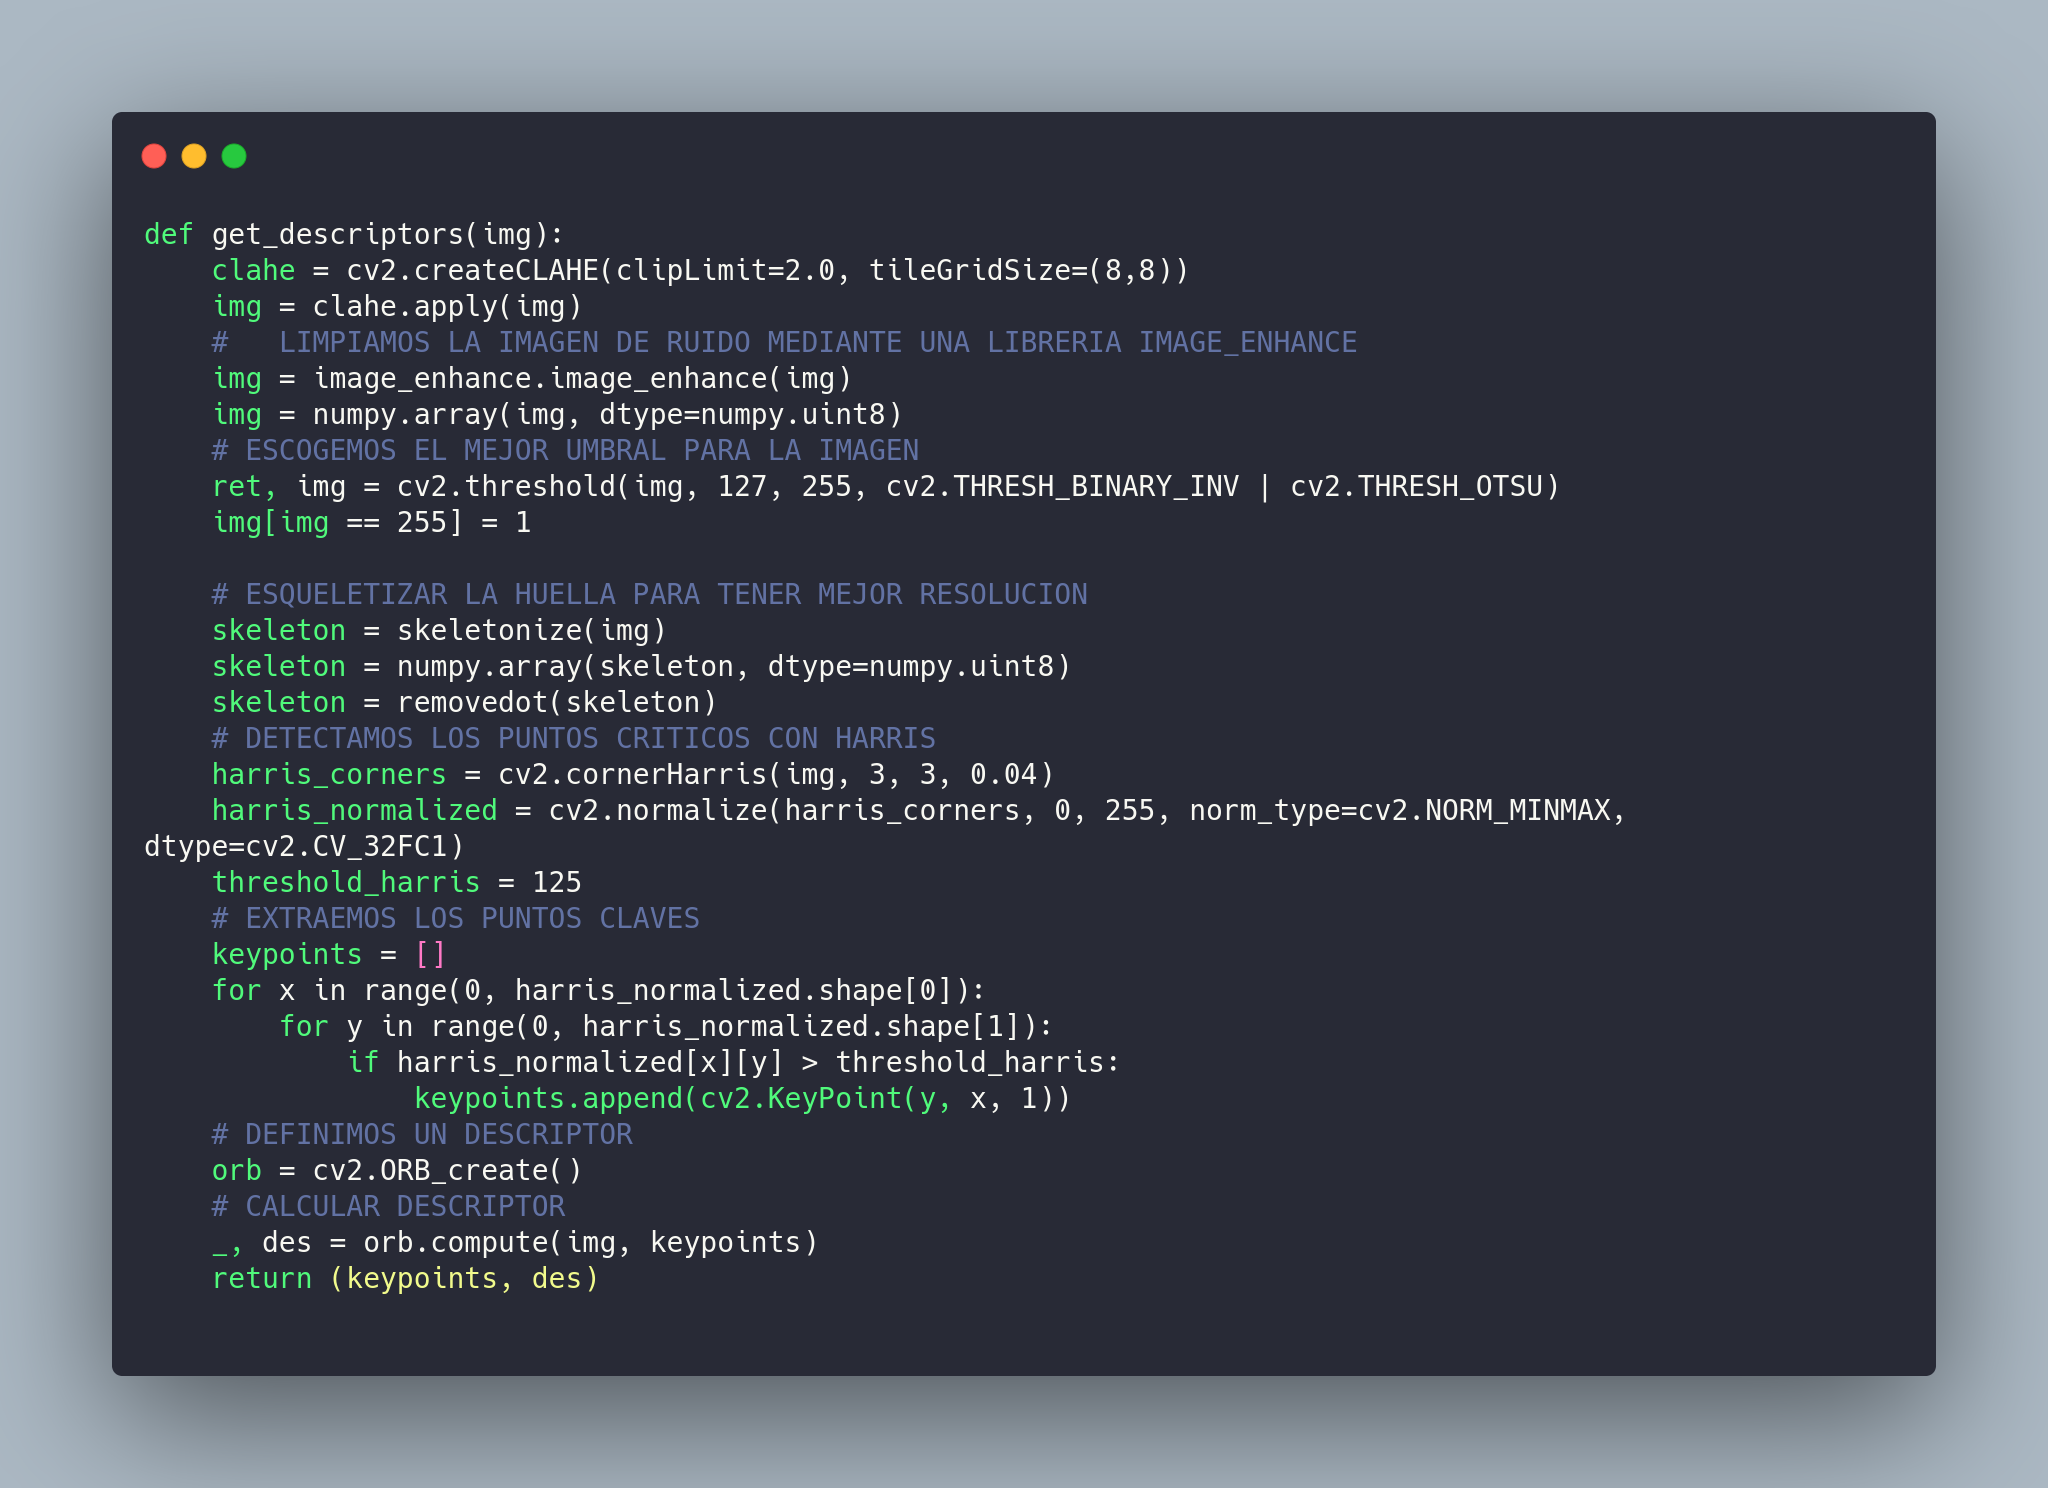
\includegraphics[width=0.4\textwidth]{./IMAGENES/descriptor}\par}
{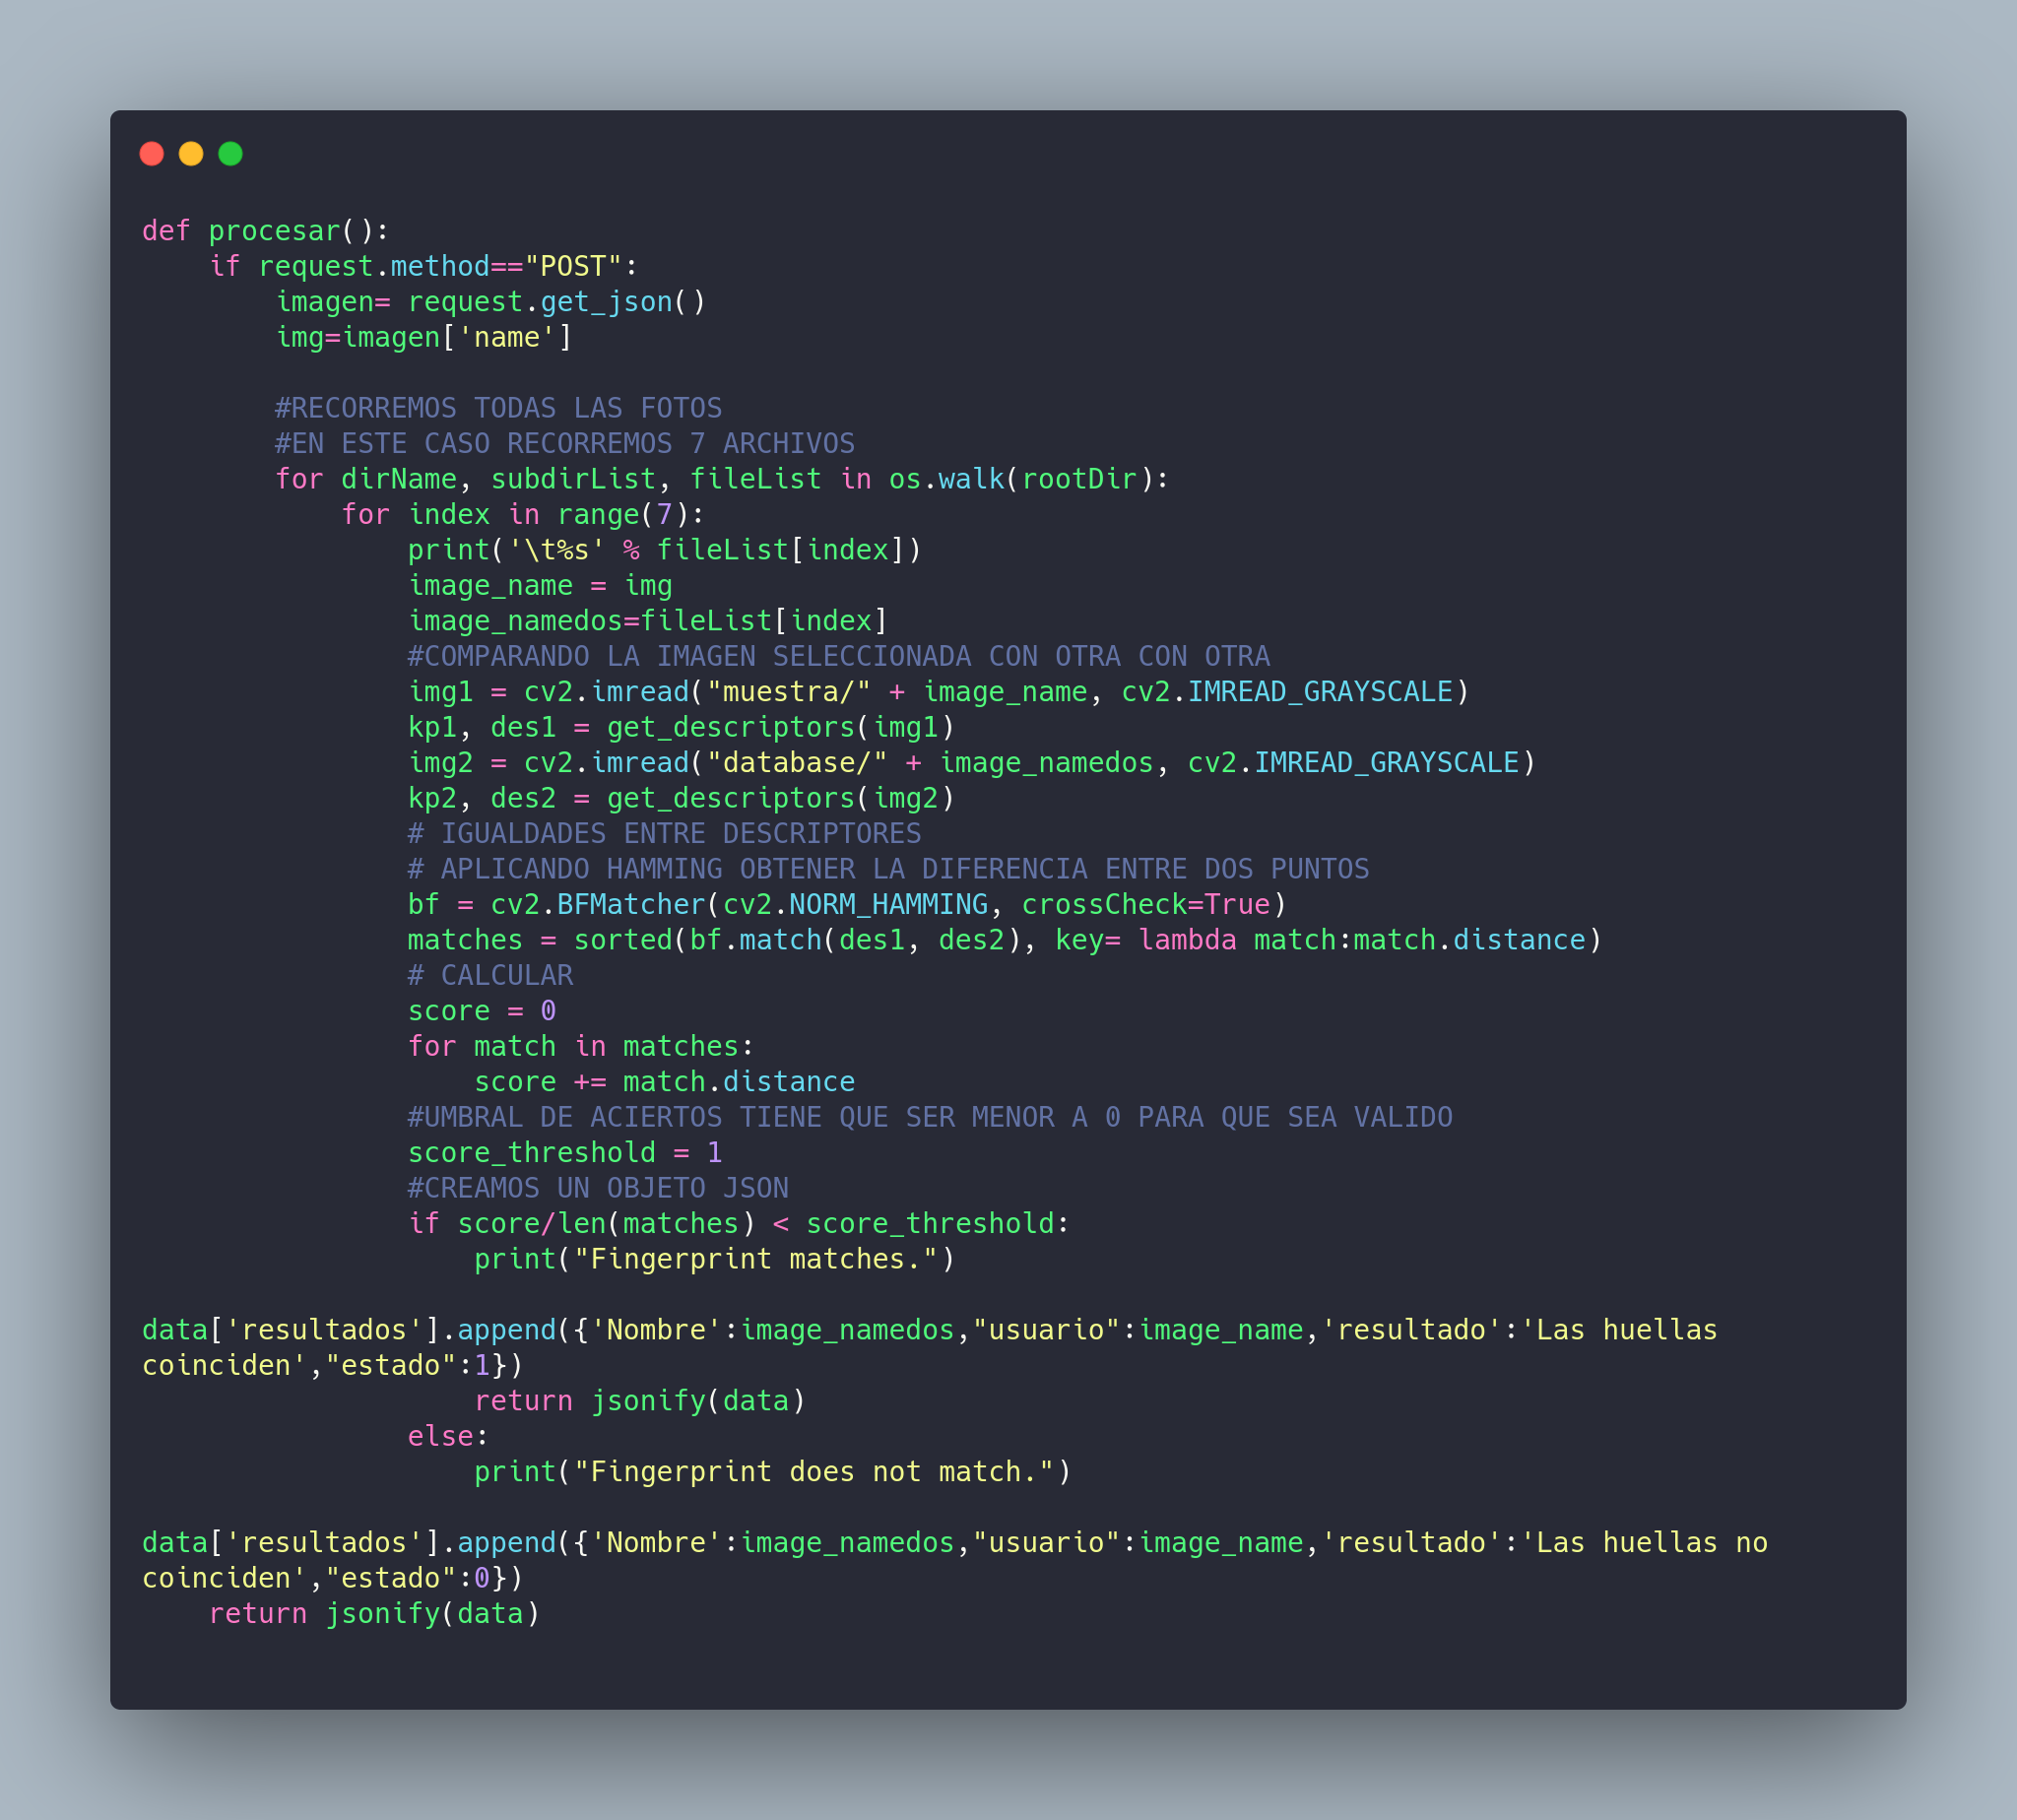
\includegraphics[width=0.4\textwidth]{./IMAGENES/procesar}\par}
%% ----------------------------------------------------------------------------------------------------------------------------------


%% Resultados------------------------------------------------------------------------------------------------------------

\section{Resultados}
	\subsection{Interfaz del sistema}
	{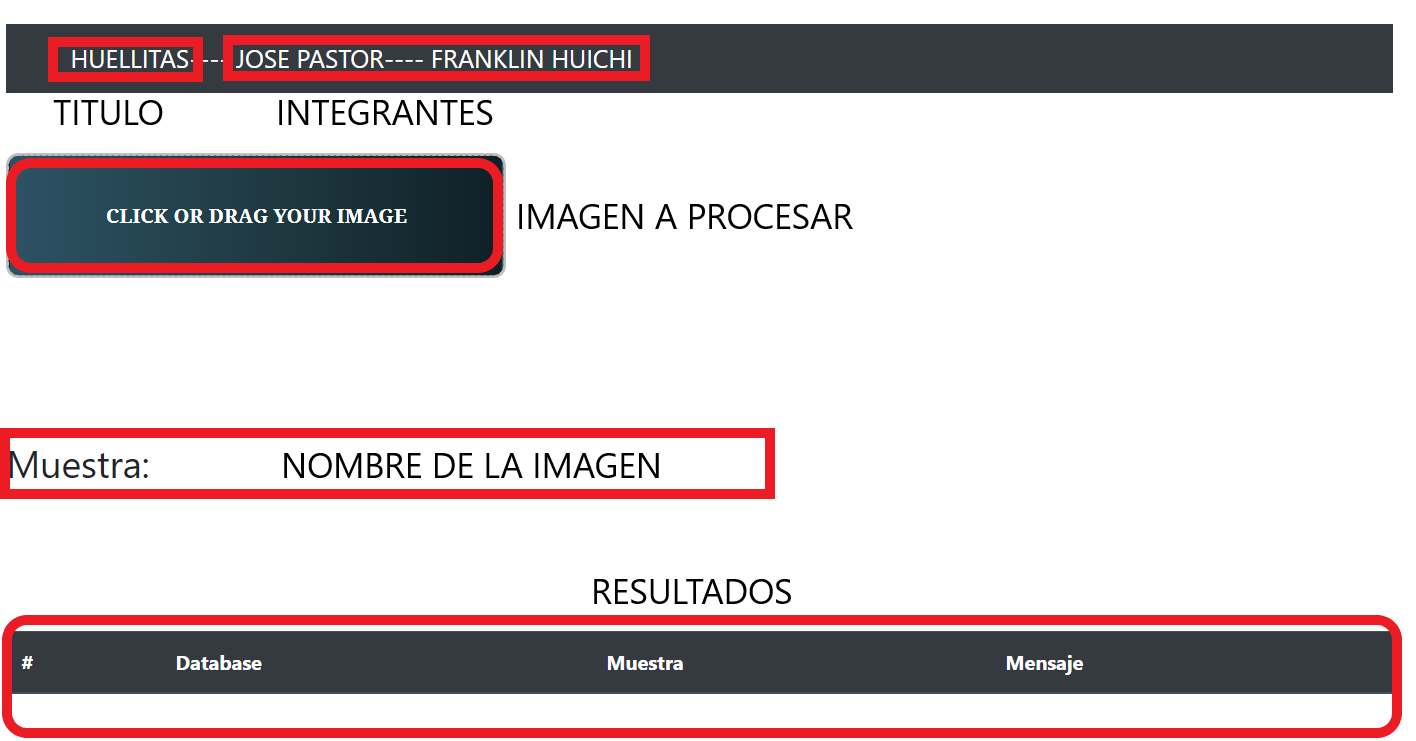
\includegraphics[width=0.4\textwidth]{./IMAGENES/interfaz}\par}
	\subsection{Base de datos de huellas dactilares .bmp}
	{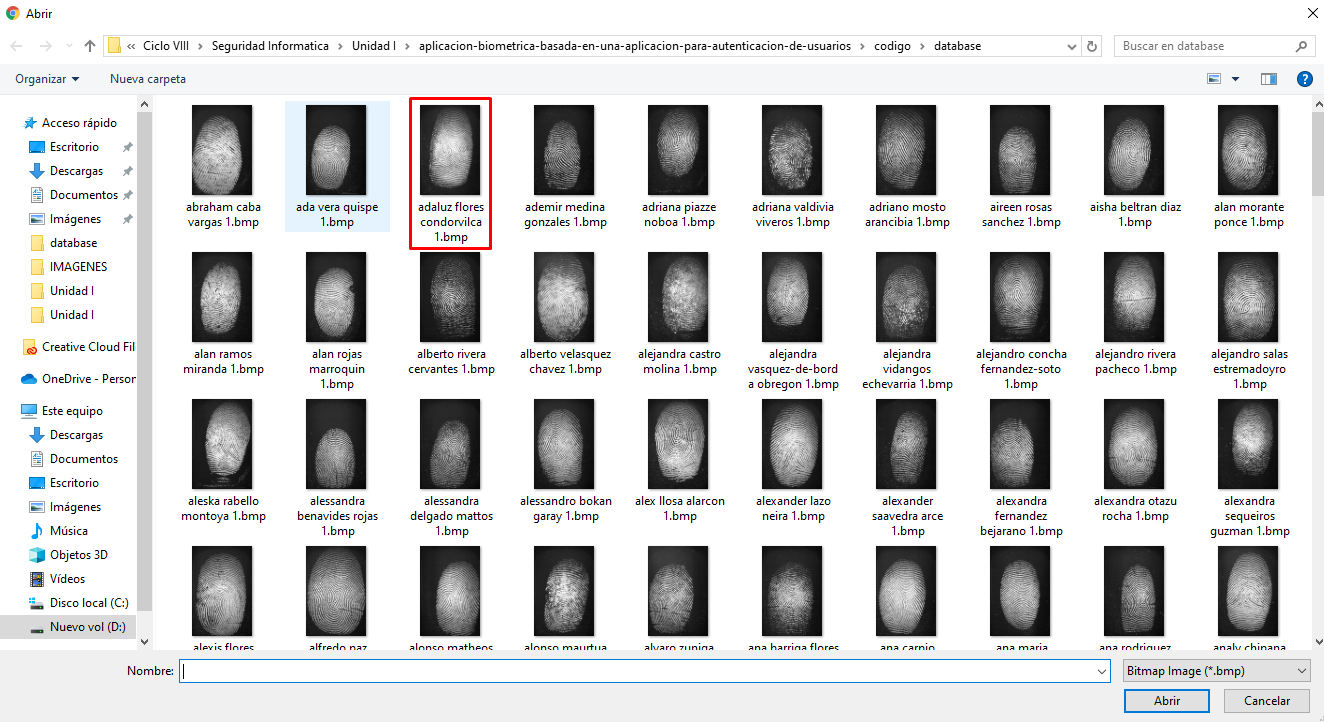
\includegraphics[width=0.4\textwidth]{./IMAGENES/huellas}\par}
	\subsection{Alerta cuando el sistema encuentra una igualdad}
	{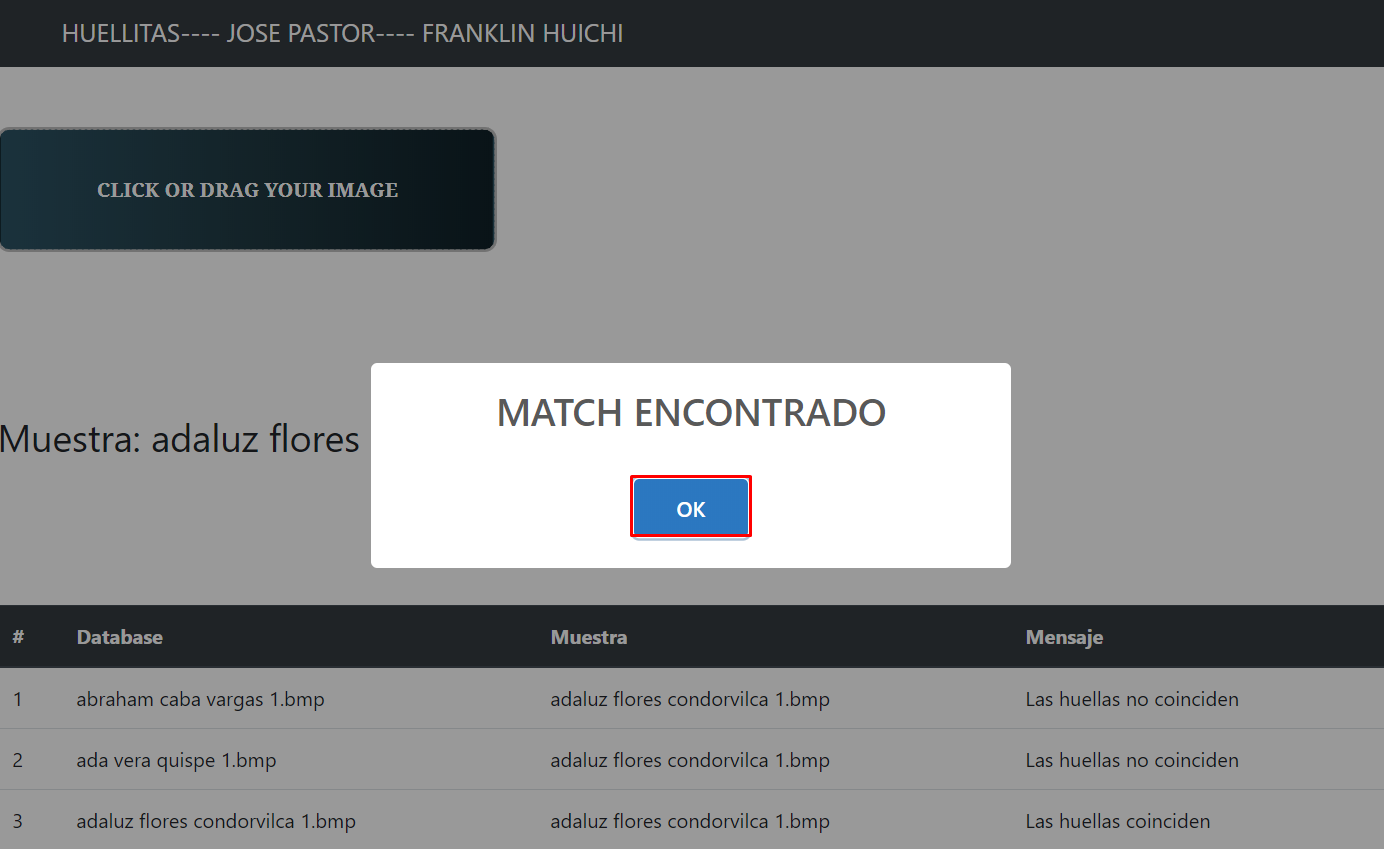
\includegraphics[width=0.4\textwidth]{./IMAGENES/match}\par}
%%Ejemplo de cita



%% ----------------------------------------------------------------------------------------------------------------------------------


%% CONCLUSIONES ---------------------------------------------------------------------------------------------------------------

\section{Conclusiones}

\begin{itemize}

\item Conclusion 1 : \\
En conclusion aprendimos a usar la tecnlogia OpenCV y Python en el rubro de la biometrica alcanzado el objetivo de encontrar huellas en el banco de imagenes usadas como muestras.
\item Conclusion 2 : \\ 
Con este proyecto, se desarrolló un sistema de reconocimiento de huellas digitales basado en el método de búsqueda de puntos críticos. Estos puntos se utilizan para encontrar descriptores formales de la región que los rodea, formando una matriz que identifica la huella en sí. Probé el sistema en el conjunto de datos FCV2002 DB1 para determinar si estaba reconociendo correctamente las impresiones.
\item Conclusion 3 : \\ 
Durante el desarrollo del sistema aprendimos y comprendimos mejor la biometria dactilar, ademas de integrar tecnologias backend (python) y de frontend(vuejs) para lograr un mejor funcionamiento. 
\end{itemize}
%%\cite{Gartner} 
%% ----------------------------------------------------------------------------------------------------------------------------------
\end{multicols}

%%  REFERENCIAS BIBLIOGRÁFICAS ------------------------------------------------------------------------------------------
	
	%%\newpage
	
	%%\bibliographystyle{apalike} 	%ESTILO
	%%\bibliography{BIBLIOGRAFIA}	 

\end{document}
